\documentclass{article}
\usepackage {nopageno}
\usepackage{caption}
\usepackage{subcaption}
\usepackage{tikz}
\usetikzlibrary{bayesnet}
\usepackage{graphicx}

\begin{document}
    \begin{figure}
         \vspace{-2cm}
         \begin{subfigure}{\textwidth}
             \hspace{-3.0cm}
             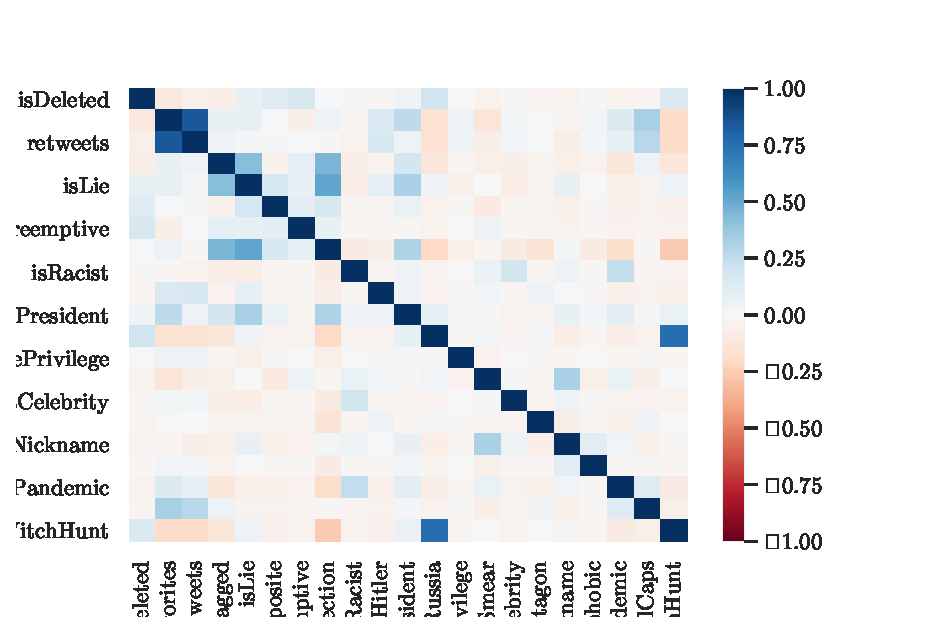
\includegraphics{corr_heatmap.eps}
             \caption{Matrix visualization of Pearson\'s correlation coefficient.}
         \end{subfigure}
         \vspace{2cm}
         \begin{subfigure}{\textwidth}
             \hspace{-.6cm}
             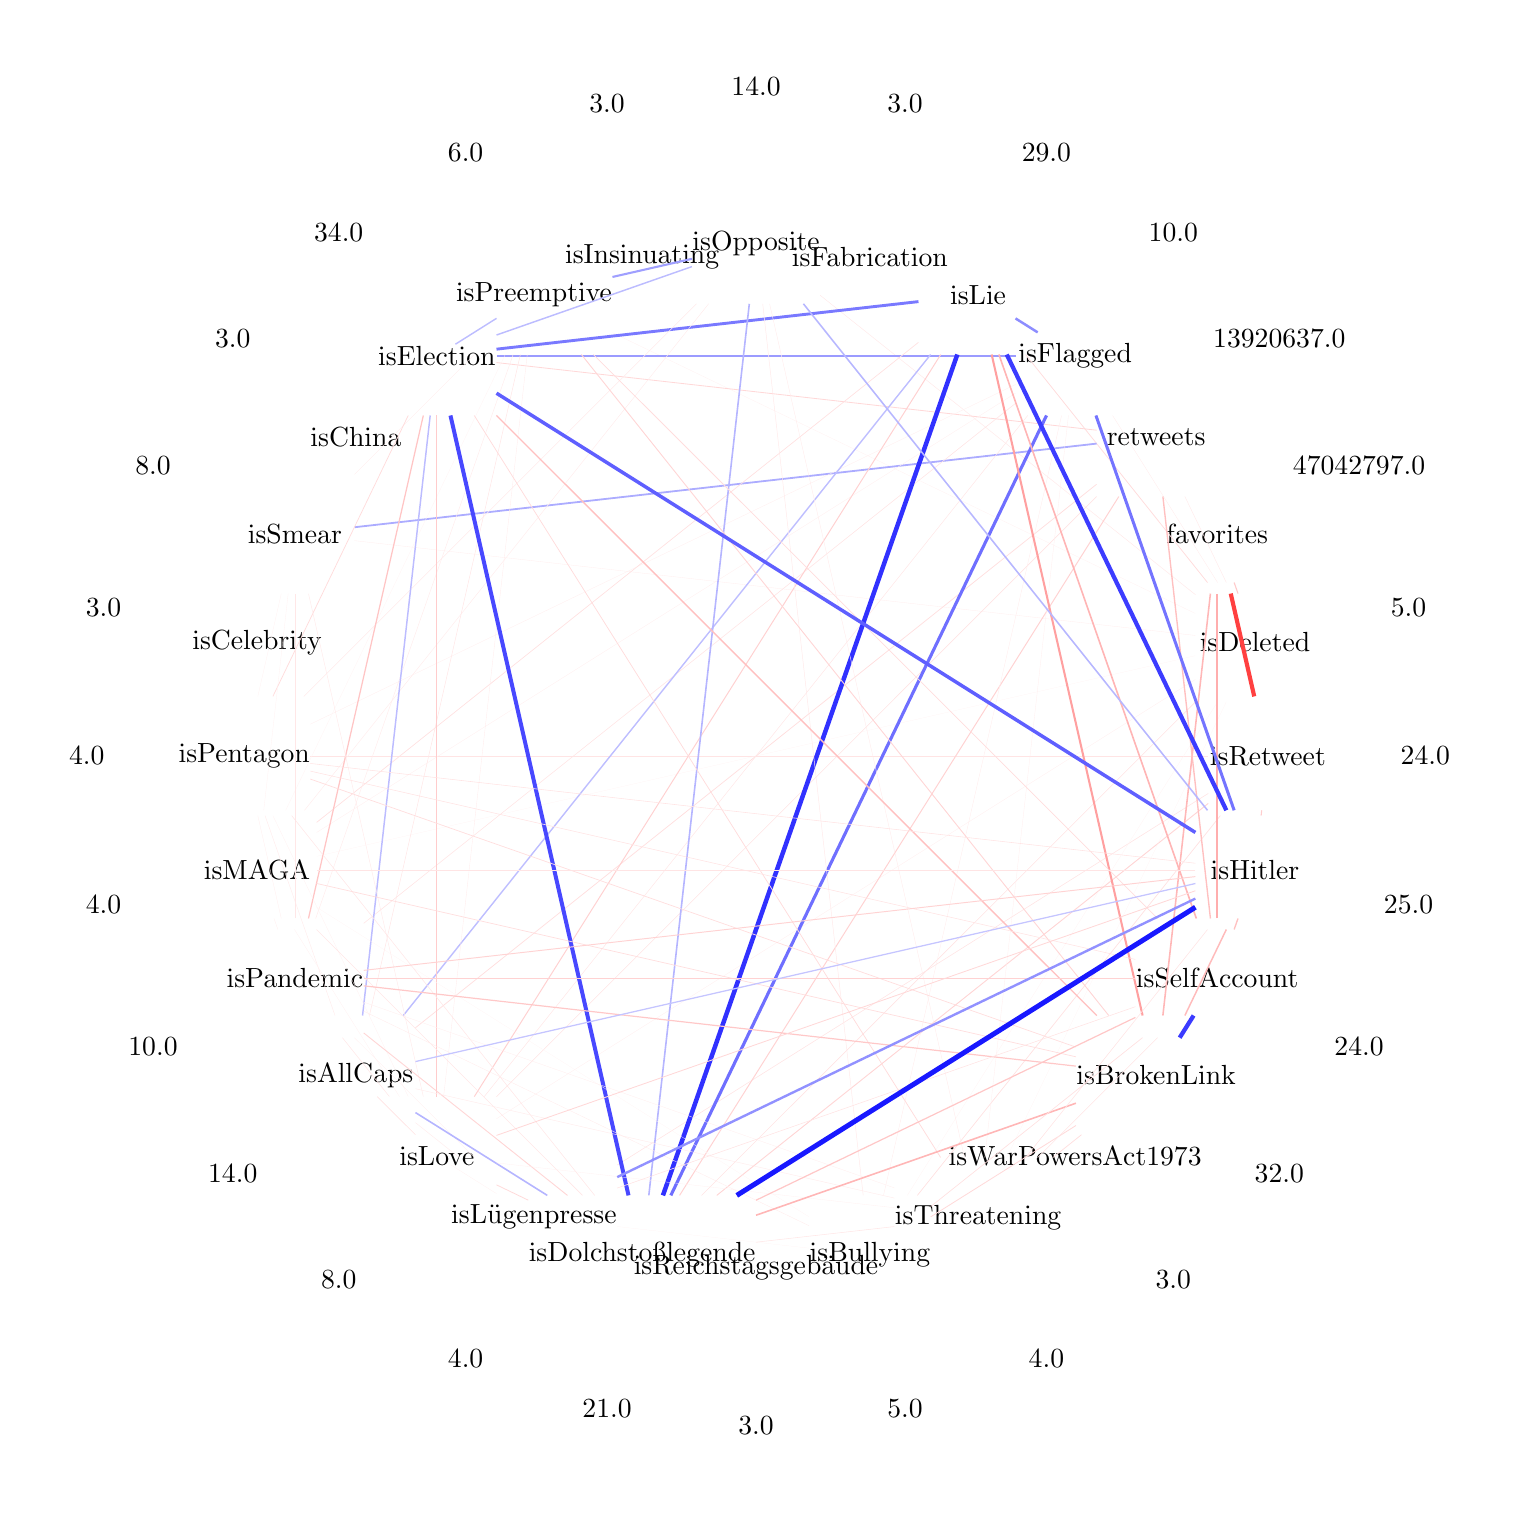
\begin{tikzpicture}
\node[const] (isRetweet) [xshift=6.500000000000000cm, yshift=0.000000000000000cm, minimum size=1.5cm] {isRetweet}; \node[const] (isDeleted) [xshift=6.337031429181853cm, yshift=1.446386070716044cm, minimum size=1.5cm] {isDeleted}; \node[const] (favorites) [xshift=5.856297641365725cm, yshift=2.820244304264128cm, minimum size=1.5cm] {favorites}; \node[const] (retweets) [xshift=5.081904636042194cm, yshift=4.052683712081768cm, minimum size=1.5cm] {retweets}; \node[const] (isFlagged) [xshift=4.052683712081769cm, yshift=5.081904636042194cm, minimum size=1.5cm] {isFlagged}; \node[const] (isLie) [xshift=2.820244304264128cm, yshift=5.856297641365725cm, minimum size=1.5cm] {isLie}; \node[const] (isFabrication) [xshift=1.446386070716044cm, yshift=6.337031429181853cm, minimum size=1.5cm] {isFabrication}; \node[const] (isOpposite) [xshift=0.000000000000000cm, yshift=6.500000000000000cm, minimum size=1.5cm] {isOpposite}; \node[const] (isInsinuating) [xshift=-1.446386070716043cm, yshift=6.337031429181853cm, minimum size=1.5cm] {isInsinuating}; \node[const] (isPreemptive) [xshift=-2.820244304264127cm, yshift=5.856297641365725cm, minimum size=1.5cm] {isPreemptive}; \node[const] (isElection) [xshift=-4.052683712081768cm, yshift=5.081904636042195cm, minimum size=1.5cm] {isElection}; \node[const] (isChina) [xshift=-5.081904636042194cm, yshift=4.052683712081769cm, minimum size=1.5cm] {isChina}; \node[const] (isSmear) [xshift=-5.856297641365724cm, yshift=2.820244304264128cm, minimum size=1.5cm] {isSmear}; \node[const] (isCelebrity) [xshift=-6.337031429181853cm, yshift=1.446386070716044cm, minimum size=1.5cm] {isCelebrity}; \node[const] (isPentagon) [xshift=-6.500000000000000cm, yshift=0.000000000000001cm, minimum size=1.5cm] {isPentagon}; \node[const] (isMAGA) [xshift=-6.337031429181853cm, yshift=-1.446386070716043cm, minimum size=1.5cm] {isMAGA}; \node[const] (isPandemic) [xshift=-5.856297641365725cm, yshift=-2.820244304264127cm, minimum size=1.5cm] {isPandemic}; \node[const] (isAllCaps) [xshift=-5.081904636042195cm, yshift=-4.052683712081767cm, minimum size=1.5cm] {isAllCaps}; \node[const] (isLove) [xshift=-4.052683712081769cm, yshift=-5.081904636042193cm, minimum size=1.5cm] {isLove}; \node[const] (isLügenpresse) [xshift=-2.820244304264129cm, yshift=-5.856297641365724cm, minimum size=1.5cm] {isLügenpresse}; \node[const] (isDolchstoßlegende) [xshift=-1.446386070716045cm, yshift=-6.337031429181853cm, minimum size=1.5cm] {isDolchstoßlegende}; \node[const] (isReichstagsgebäude) [xshift=-0.000000000000001cm, yshift=-6.500000000000000cm, minimum size=1.5cm] {isReichstagsgebäude}; \node[const] (isBullying) [xshift=1.446386070716043cm, yshift=-6.337031429181853cm, minimum size=1.5cm] {isBullying}; \node[const] (isThreatening) [xshift=2.820244304264127cm, yshift=-5.856297641365726cm, minimum size=1.5cm] {isThreatening}; \node[const] (isWarPowersAct1973) [xshift=4.052683712081767cm, yshift=-5.081904636042195cm, minimum size=1.5cm] {isWarPowersAct1973}; \node[const] (isBrokenLink) [xshift=5.081904636042193cm, yshift=-4.052683712081769cm, minimum size=1.5cm] {isBrokenLink}; \node[const] (isSelfAccount) [xshift=5.856297641365724cm, yshift=-2.820244304264129cm, minimum size=1.5cm] {isSelfAccount}; \node[const] (isHitler) [xshift=6.337031429181852cm, yshift=-1.446386070716045cm, minimum size=1.5cm] {isHitler}; \node[const] (24.0) [xshift=8.500000000000000cm, yshift=0.000000000000000cm, minimum size=1.5cm] {24.0}; \node[const] (5.0) [xshift=8.286887253545501cm, yshift=1.891427938628672cm, minimum size=1.5cm] {5.0}; \node[const] (47042797.0) [xshift=7.658235377170563cm, yshift=3.688011782499244cm, minimum size=1.5cm] {47042797.0}; \node[const] (13920637.0) [xshift=6.645567600978254cm, yshift=5.299663315799235cm, minimum size=1.5cm] {13920637.0}; \node[const] (10.0) [xshift=5.299663315799235cm, yshift=6.645567600978254cm, minimum size=1.5cm] {10.0}; \node[const] (29.0) [xshift=3.688011782499244cm, yshift=7.658235377170563cm, minimum size=1.5cm] {29.0}; \node[const] (3.0) [xshift=1.891427938628673cm, yshift=8.286887253545501cm, minimum size=1.5cm] {3.0}; \node[const] (14.0) [xshift=0.000000000000001cm, yshift=8.500000000000000cm, minimum size=1.5cm] {14.0}; \node[const] (3.0) [xshift=-1.891427938628672cm, yshift=8.286887253545501cm, minimum size=1.5cm] {3.0}; \node[const] (6.0) [xshift=-3.688011782499244cm, yshift=7.658235377170563cm, minimum size=1.5cm] {6.0}; \node[const] (34.0) [xshift=-5.299663315799235cm, yshift=6.645567600978254cm, minimum size=1.5cm] {34.0}; \node[const] (3.0) [xshift=-6.645567600978254cm, yshift=5.299663315799235cm, minimum size=1.5cm] {3.0}; \node[const] (8.0) [xshift=-7.658235377170562cm, yshift=3.688011782499245cm, minimum size=1.5cm] {8.0}; \node[const] (3.0) [xshift=-8.286887253545501cm, yshift=1.891427938628673cm, minimum size=1.5cm] {3.0}; \node[const] (4.0) [xshift=-8.500000000000000cm, yshift=0.000000000000001cm, minimum size=1.5cm] {4.0}; \node[const] (4.0) [xshift=-8.286887253545501cm, yshift=-1.891427938628671cm, minimum size=1.5cm] {4.0}; \node[const] (10.0) [xshift=-7.658235377170563cm, yshift=-3.688011782499243cm, minimum size=1.5cm] {10.0}; \node[const] (14.0) [xshift=-6.645567600978254cm, yshift=-5.299663315799234cm, minimum size=1.5cm] {14.0}; \node[const] (8.0) [xshift=-5.299663315799236cm, yshift=-6.645567600978253cm, minimum size=1.5cm] {8.0}; \node[const] (4.0) [xshift=-3.688011782499245cm, yshift=-7.658235377170562cm, minimum size=1.5cm] {4.0}; \node[const] (21.0) [xshift=-1.891427938628674cm, yshift=-8.286887253545501cm, minimum size=1.5cm] {21.0}; \node[const] (3.0) [xshift=-0.000000000000002cm, yshift=-8.500000000000000cm, minimum size=1.5cm] {3.0}; \node[const] (5.0) [xshift=1.891427938628671cm, yshift=-8.286887253545501cm, minimum size=1.5cm] {5.0}; \node[const] (4.0) [xshift=3.688011782499243cm, yshift=-7.658235377170564cm, minimum size=1.5cm] {4.0}; \node[const] (3.0) [xshift=5.299663315799234cm, yshift=-6.645567600978254cm, minimum size=1.5cm] {3.0}; \node[const] (32.0) [xshift=6.645567600978253cm, yshift=-5.299663315799236cm, minimum size=1.5cm] {32.0}; \node[const] (24.0) [xshift=7.658235377170562cm, yshift=-3.688011782499246cm, minimum size=1.5cm] {24.0}; \node[const] (25.0) [xshift=8.286887253545499cm, yshift=-1.891427938628675cm, minimum size=1.5cm] {25.0}; \edge [-, color=red!75.03525076303045!white, line width=1.500705015260609pt] {favorites} {isRetweet}; \edge [-, color=red!20.62976432956229!white, line width=0.412595286591246pt] {favorites} {isDeleted}; \edge [-, color=red!8.190814620236678!white, line width=0.163816292404734pt] {retweets} {isDeleted}; \edge [-, color=red!7.124966946226453!white, line width=0.142499338924529pt] {isFlagged} {isDeleted}; \edge [-, color=red!13.703722206983118!white, line width=0.274074444139662pt] {isLie} {isDeleted}; \edge [-, color=blue!44.73595669741125!white, line width=0.894719133948225pt] {isLie} {isFlagged}; \edge [-, color=red!8.626903606346962!white, line width=0.172538072126939pt] {isOpposite} {isDeleted}; \edge [-, color=red!5.3469716814441455!white, line width=0.106939433628883pt] {isPreemptive} {isDeleted}; \edge [-, color=blue!37.689161824688405!white, line width=0.753783236493768pt] {isPreemptive} {isOpposite}; \edge [-, color=red!15.10591379463353!white, line width=0.302118275892671pt] {isElection} {retweets}; \edge [-, color=blue!39.38994245445259!white, line width=0.787798849089052pt] {isElection} {isFlagged}; \edge [-, color=blue!52.37835864148476!white, line width=1.047567172829695pt] {isElection} {isLie}; \edge [-, color=blue!26.277645705644893!white, line width=0.525552914112898pt] {isElection} {isOpposite}; \edge [-, color=blue!25.915604951372618!white, line width=0.518312099027452pt] {isElection} {isPreemptive}; \edge [-, color=red!6.268348052757345!white, line width=0.125366961055147pt] {isSmear} {isDeleted}; \edge [-, color=blue!32.4838907214276!white, line width=0.649677814428552pt] {isSmear} {retweets}; \edge [-, color=red!6.949097855051053!white, line width=0.138981957101021pt] {isSmear} {isPreemptive}; \edge [-, color=red!10.716171282173148!white, line width=0.214323425643463pt] {isPentagon} {isRetweet}; \edge [-, color=red!6.323191507049368!white, line width=0.126463830140987pt] {isPentagon} {isFlagged}; \edge [-, color=red!7.64863055334671!white, line width=0.152972611066934pt] {isPentagon} {isOpposite}; \edge [-, color=red!13.650447497876645!white, line width=0.273008949957533pt] {isPentagon} {isElection}; \edge [-, color=red!5.554904893073856!white, line width=0.111098097861477pt] {isPentagon} {isSmear}; \edge [-, color=red!4.283336727363114!white, line width=0.085666734547262pt] {isMAGA} {isDeleted}; \edge [-, color=red!6.330116757901437!white, line width=0.126602335158029pt] {isMAGA} {isFlagged}; \edge [-, color=red!12.180435746565506!white, line width=0.243608714931310pt] {isMAGA} {isLie}; \edge [-, color=red!7.664646508917474!white, line width=0.153292930178349pt] {isMAGA} {isOpposite}; \edge [-, color=red!4.756192303367214!white, line width=0.095123846067344pt] {isMAGA} {isPreemptive}; \edge [-, color=red!5.569048010060512!white, line width=0.111380960201210pt] {isMAGA} {isSmear}; \edge [-, color=red!10.499033234087488!white, line width=0.209980664681750pt] {isPandemic} {isFlagged}; \edge [-, color=red!7.885811771133606!white, line width=0.157716235422672pt] {isPandemic} {isPreemptive}; \edge [-, color=red!22.681514742059594!white, line width=0.453630294841192pt] {isPandemic} {isElection}; \edge [-, color=red!9.24397714828555!white, line width=0.184879542965711pt] {isPandemic} {isSmear}; \edge [-, color=red!6.303263564638281!white, line width=0.126065271292766pt] {isPandemic} {isPentagon}; \edge [-, color=red!6.312289865471206!white, line width=0.126245797309424pt] {isPandemic} {isMAGA}; \edge [-, color=red!13.097932885307802!white, line width=0.261958657706156pt] {isAllCaps} {retweets}; \edge [-, color=blue!25.468567060320197!white, line width=0.509371341206404pt] {isAllCaps} {isLie}; \edge [-, color=red!9.601217475425404!white, line width=0.192024349508508pt] {isAllCaps} {isPreemptive}; \edge [-, color=blue!26.395698027881913!white, line width=0.527913960557638pt] {isAllCaps} {isElection}; \edge [-, color=red!7.675477810277807!white, line width=0.153509556205556pt] {isAllCaps} {isPentagon}; \edge [-, color=red!6.284558008094655!white, line width=0.125691160161893pt] {isLove} {isDeleted}; \edge [-, color=red!10.923687903423092!white, line width=0.218473758068462pt] {isLove} {retweets}; \edge [-, color=red!9.290808772402869!white, line width=0.185816175448057pt] {isLove} {isFlagged}; \edge [-, color=red!17.8735940993974!white, line width=0.357471881987948pt] {isLove} {isLie}; \edge [-, color=red!6.969604665151924!white, line width=0.139392093303038pt] {isLove} {isPreemptive}; \edge [-, color=red!20.066900256705583!white, line width=0.401338005134112pt] {isLove} {isElection}; \edge [-, color=red!8.17441321349957!white, line width=0.163488264269991pt] {isLove} {isSmear}; \edge [-, color=red!5.571966466226716!white, line width=0.111439329324534pt] {isLove} {isPentagon}; \edge [-, color=red!5.586564253358536!white, line width=0.111731285067171pt] {isLove} {isMAGA}; \edge [-, color=red!9.259651230409213!white, line width=0.185193024608184pt] {isLove} {isPandemic}; \edge [-, color=red!11.291213204627313!white, line width=0.225824264092546pt] {isLove} {isAllCaps}; \edge [-, color=red!10.696616231848923!white, line width=0.213932324636978pt] {isLügenpresse} {isRetweet}; \edge [-, color=red!6.287733740220119!white, line width=0.125754674804402pt] {isLügenpresse} {isPandemic}; \edge [-, color=red!7.655508428285899!white, line width=0.153110168565718pt] {isLügenpresse} {isAllCaps}; \edge [-, color=red!5.559886730330063!white, line width=0.111197734606601pt] {isLügenpresse} {isLove}; \edge [-, color=red!16.441047206236938!white, line width=0.328820944124739pt] {isDolchstoßlegende} {isRetweet}; \edge [-, color=red!11.058511112169024!white, line width=0.221170222243380pt] {isDolchstoßlegende} {isDeleted}; \edge [-, color=red!17.82730202441965!white, line width=0.356546040488393pt] {isDolchstoßlegende} {retweets}; \edge [-, color=blue!56.28550227543185!white, line width=1.125710045508637pt] {isDolchstoßlegende} {isFlagged}; \edge [-, color=blue!80.74654888892402!white, line width=1.614930977778481pt] {isDolchstoßlegende} {isLie}; \edge [-, color=blue!28.970390285036977!white, line width=0.579407805700740pt] {isDolchstoßlegende} {isOpposite}; \edge [-, color=blue!71.948424332311!white, line width=1.438968486646220pt] {isDolchstoßlegende} {isElection}; \edge [-, color=red!9.81569193688276!white, line width=0.196313838737655pt] {isDolchstoßlegende} {isPentagon}; \edge [-, color=red!9.830562917244842!white, line width=0.196611258344897pt] {isDolchstoßlegende} {isMAGA}; \edge [-, color=red!16.300414674959598!white, line width=0.326008293499192pt] {isDolchstoßlegende} {isPandemic}; \edge [-, color=blue!29.06057279574677!white, line width=0.581211455914935pt] {isDolchstoßlegende} {isAllCaps}; \edge [-, color=red!14.423714450269864!white, line width=0.288474289005397pt] {isDolchstoßlegende} {isLove}; \edge [-, color=red!12.169345012988769!white, line width=0.243386900259775pt] {isBullying} {isRetweet}; \edge [-, color=red!4.8531902227490855!white, line width=0.097063804454982pt] {isBullying} {isDeleted}; \edge [-, color=red!7.178326223077118!white, line width=0.143566524461542pt] {isBullying} {isFlagged}; \edge [-, color=red!8.685906193982108!white, line width=0.173718123879642pt] {isBullying} {isOpposite}; \edge [-, color=red!4.314834566158357!white, line width=0.086296691323167pt] {isBullying} {isMAGA}; \edge [-, color=red!7.162065483535039!white, line width=0.143241309670701pt] {isBullying} {isPandemic}; \edge [-, color=red!4.299197182809307!white, line width=0.085983943656186pt] {isBullying} {isLügenpresse}; \edge [-, color=red!4.272283476112053!white, line width=0.085445669522241pt] {isThreatening} {isDeleted}; \edge [-, color=red!6.312566955248025!white, line width=0.126251339104961pt] {isThreatening} {isFlagged}; \edge [-, color=red!7.642184118724243!white, line width=0.152843682374485pt] {isThreatening} {isOpposite}; \edge [-, color=red!13.632731854574173!white, line width=0.272654637091483pt] {isThreatening} {isElection}; \edge [-, color=red!6.303202877790917!white, line width=0.126064057555818pt] {isThreatening} {isPandemic}; \edge [-, color=red!7.671815670669324!white, line width=0.153436313413386pt] {isThreatening} {isAllCaps}; \edge [-, color=red!5.568626736363347!white, line width=0.111372534727267pt] {isThreatening} {isLove}; \edge [-, color=red!9.801567082848663!white, line width=0.196031341656973pt] {isThreatening} {isDolchstoßlegende}; \edge [-, color=red!28.125143973703437!white, line width=0.562502879474069pt] {isBrokenLink} {favorites}; \edge [-, color=red!37.15750690078076!white, line width=0.743150138015615pt] {isBrokenLink} {isLie}; \edge [-, color=red!16.319668867264888!white, line width=0.326393377345298pt] {isBrokenLink} {isPreemptive}; \edge [-, color=red!24.80112748458216!white, line width=0.496022549691643pt] {isBrokenLink} {isElection}; \edge [-, color=red!13.05368433888269!white, line width=0.261073686777654pt] {isBrokenLink} {isPentagon}; \edge [-, color=red!13.080565134889651!white, line width=0.261611302697793pt] {isBrokenLink} {isMAGA}; \edge [-, color=red!21.687146564473764!white, line width=0.433742931289475pt] {isBrokenLink} {isPandemic}; \edge [-, color=red!28.555714672751353!white, line width=0.571114293455027pt] {isBrokenLink} {isDolchstoßlegende}; \edge [-, color=red!14.816892110982261!white, line width=0.296337842219645pt] {isBrokenLink} {isBullying}; \edge [-, color=red!13.039071333391064!white, line width=0.260781426667821pt] {isBrokenLink} {isThreatening}; \edge [-, color=red!31.87983330274736!white, line width=0.637596666054947pt] {isSelfAccount} {favorites}; \edge [-, color=red!24.876748988322838!white, line width=0.497534979766457pt] {isSelfAccount} {retweets}; \edge [-, color=red!29.206514720568688!white, line width=0.584130294411374pt] {isSelfAccount} {isLie}; \edge [-, color=red!13.382276075498641!white, line width=0.267645521509973pt] {isSelfAccount} {isPreemptive}; \edge [-, color=red!10.70319148953922!white, line width=0.214063829790784pt] {isSelfAccount} {isPentagon}; \edge [-, color=red!17.78373821187645!white, line width=0.355674764237529pt] {isSelfAccount} {isPandemic}; \edge [-, color=red!10.680784290511768!white, line width=0.213615685810235pt] {isSelfAccount} {isLügenpresse}; \edge [-, color=red!22.006158926387894!white, line width=0.440123178527758pt] {isSelfAccount} {isDolchstoßlegende}; \edge [-, color=red!12.149709470318761!white, line width=0.242994189406375pt] {isSelfAccount} {isBullying}; \edge [-, color=red!10.69196222448346!white, line width=0.213839244489669pt] {isSelfAccount} {isThreatening}; \edge [-, color=blue!77.03045530202303!white, line width=1.540609106040461pt] {isSelfAccount} {isBrokenLink}; \edge [-, color=red!19.46182605808525!white, line width=0.389236521161705pt] {isHitler} {isRetweet}; \edge [-, color=blue!54.39927288219859!white, line width=1.087985457643972pt] {isHitler} {isFlagged}; \edge [-, color=blue!76.55385446796764!white, line width=1.531077089359353pt] {isHitler} {isLie}; \edge [-, color=blue!28.37354762791161!white, line width=0.567470952558232pt] {isHitler} {isOpposite}; \edge [-, color=blue!62.91521190056264!white, line width=1.258304238011253pt] {isHitler} {isElection}; \edge [-, color=red!10.490841671806548!white, line width=0.209816833436131pt] {isHitler} {isPentagon}; \edge [-, color=red!10.506189774794734!white, line width=0.210123795495895pt] {isHitler} {isMAGA}; \edge [-, color=red!17.419751616812302!white, line width=0.348395032336246pt] {isHitler} {isPandemic}; \edge [-, color=blue!22.793800957499748!white, line width=0.455876019149995pt] {isHitler} {isAllCaps}; \edge [-, color=red!15.409244293503965!white, line width=0.308184885870079pt] {isHitler} {isLove}; \edge [-, color=blue!42.994478675061835!white, line width=0.859889573501237pt] {isHitler} {isLügenpresse}; \edge [-, color=blue!90.45701251489112!white, line width=1.809140250297822pt] {isHitler} {isDolchstoßlegende}; \edge [-, color=red!10.475605628060947!white, line width=0.209512112561219pt] {isHitler} {isThreatening}; \edge [-, color=red!26.722093897670167!white, line width=0.534441877953403pt] {isHitler} {isBrokenLink}; \edge [-, color=red!24.466846014412635!white, line width=0.489336920288253pt] {isHitler} {isSelfAccount}; 
\end{tikzpicture}
             \caption{Graph visualization of Pearson\'s correlation coefficient. Blue means a positive linear relationship between the two, red is a negative relationship.}
         \end{subfigure}
    \end{figure}

\end{document}